\documentclass[12pt]{article}
\usepackage{graphicx}

\textwidth 15.2cm
\textheight 22.0cm
\topmargin  -1.5cm
\oddsidemargin 0.5cm
\evensidemargin 0.5cm
\pagestyle{empty}

%\partopsep -33pt
%\parsep 0pt
%\topskip -33pt
\parskip 0pt
\parindent 0pt
\setlength{\topsep}{0pt}
\setlength{\partopsep}{0pt}
\setlength{\itemsep}{-30pt}
\setlength{\parsep}{-30pt}

\makeatletter
   \def\@listi{\itemsep0pt\parsep0pt}
\makeatother




%\renewcommand{\baselinestretch}{0.9}
\renewcommand{\topfraction}{0.8}
\renewcommand{\textfraction}{0.2}
\renewcommand{\floatpagefraction}{0.8}

%\settowidth{\leftmargin}{CC}
%\addtolength{\leftmargin}{-30pt}
%\setlength{\leftmargin}{5pt}

\begin{document}

\section*{The isovector surface term in the Fayans functional}

So far, we had not included the isovector surface term, $\propto
a_-^{(s)}(\nabla\rho_-)^2$, in the f´Fayans functional. Thus we
launched fits with free variation of $a_-^{(s)}\equiv$\texttt{asm}
starting from the Fy(IVP3) functional with finite pairing width 0.9 fm.
The straightforward fit delivered $a_-^{(s)}=0.005\pm 0.016$ well
compatible with zero. To make sure that we are not fooled by a rough
$\chi^2$ landscape, we counter-checked by a series of fits with fixed
and systematically varied \texttt{asm}.

\bigskip

\centerline{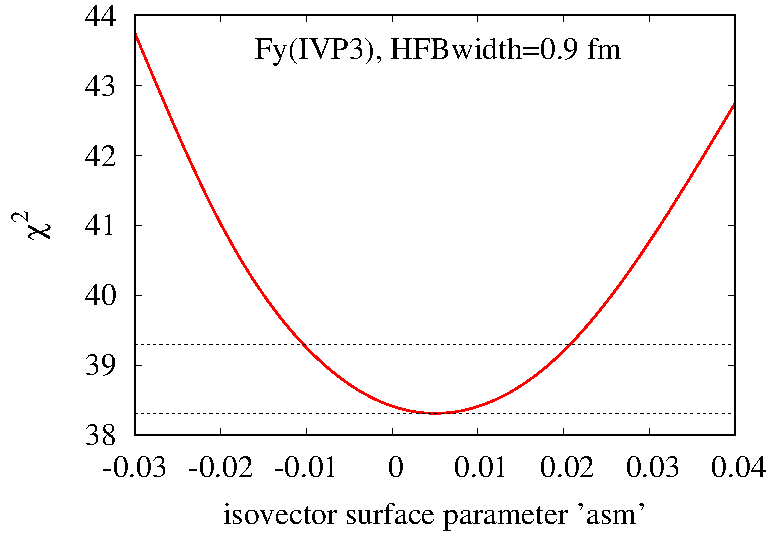
\includegraphics[width=\linewidth]{test_isovector_surface.pdf}}

\bigskip

The above figure shows the resulting $chi^2$ as function of
\texttt{asm}$\equiv a_-^{(s)}$. it confirms perfectly the findings
from the fit with free $\texttt{asm}$. The isovector surface term does
not play a helpful role. The same was found earlier in fit of Skyrme
forces where the isovector surface parameter is in most cases
compatible with zero within the $2\sigma$ band of variation. In case
of the Fayans Fy(IVP3) functional it is even less surprising. The
three isovector pairing parameters of Fy(IVP3) have already explored a
great deal of isovector freedom which, together with the finite-range
pairing, has delivered a huge gain in $chi^2$.

\end{document}
